\begin{center}
Общее представление о системе
\end{center}

\vspace{\baselineskip}

FreeHackQuest (FHQ) -- это платформа для обучения, проведения практических занятий и соревнований по компьютерной безопасности в формате тестирования на проникновение внутри среды, моделирующей работу информационной инфраструктуры организации. FHQ включает в себя учебник, различные задачи для решения, связанные с администрированием, криптографией, компьютерно-криминалистической экспертизой, стеганографией и многими дргуими направлениями информационной безопасности.\par

\begin{center}
Основные компоненты системы
\end{center}

\vspace{\baselineskip}

FreeHackQuest представляет собой клиент–серверную многофункциональную систему с подсистемами и состоит из следующих основных компонентов:
\begin{enumerate}
\item Уровень 1: Сервер -- отвечает за обработку запросов со стороны клиента.
\item Уровень 1: LXD (сервер виртуальных машин) -- предназначен для размещения контейнеров, необходимых, для изолированного выполнения сервисов с уязвимостями.
\item Уровень 1: MySQL (сервер баз данных) -- отвечает за хранение и предоставление информации.
\item Уровень 1: Клиент -- отвечает за формирование запросов подсистеме сервера и представление ответов со стороны сервера.
\item Уровень 1: Административный клиент -- отвечает за управление системой.
\end{enumerate}

\vspace{\baselineskip}

Структура системы представлена на рисунке \ref{img:1}.

\begin{figure}[h!]
        \centering
        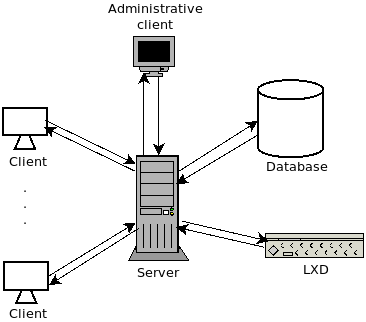
\includegraphics[width=0.65\textwidth]{1}
        \caption{Структура системы}
        \label{img:1}
\end{figure}
